% flashcards-title: Five-story building with a street door
% flashcards-desc: A building outline with five equal floor bands marked by rows of windows, and a street door at the bottom of the lowest band. No measurements are labeled.
\documentclass[dvisvgm,tikz,border=8pt]{standalone}
\usepackage{tikz}
\usetikzlibrary{arrows.meta,calc,positioning}
\definecolor{DeckInk}{HTML}{172A3A}
\definecolor{DeckAccent}{HTML}{176B87}
\definecolor{DeckWarm}{HTML}{D97706}
\definecolor{DeckMuted}{HTML}{667784}
\definecolor{DeckPaper}{HTML}{F7FAFC}
\tikzset{
  every node/.style={font=\sffamily, text=DeckInk},
  object/.style={draw=DeckInk, line width=1.1pt, fill=DeckPaper},
  primary/.style={draw=DeckAccent, line width=1.5pt},
  boundary/.style={draw=DeckAccent, line width=1.5pt, dashed, rounded corners=6pt},
  guide/.style={draw=DeckMuted, line width=0.9pt, dashed},
  dimension/.style={{Stealth[length=3.2mm,width=2.2mm]}-{Stealth[length=3.2mm,width=2.2mm]}, draw=DeckWarm, line width=1.2pt},
  motion/.style={-{Stealth[length=3.5mm,width=2.5mm]}, draw=DeckAccent, line width=1.5pt, dashed},
}

\begin{document}
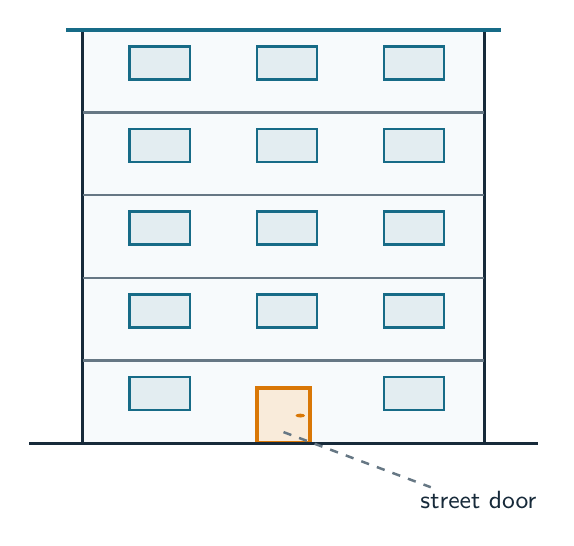
\begin{tikzpicture}[x=0.85cm,y=0.35cm]
  % Building outline
  \draw[object] (0,0) rectangle (6,15);
  % Floor-band separators
  \foreach \y in {3,6,9,12} \draw[DeckMuted, line width=0.8pt] (0,\y) -- (6,\y);
  % Roof line accent
  \draw[primary] (-0.25,15) -- (6.25,15);
  % Windows on upper floor bands (three per band)
  \foreach \y in {3,6,9,12} {
    \foreach \x in {0.7,2.6,4.5} {
      \draw[DeckAccent, line width=0.9pt, fill=DeckAccent!12]
        (\x,\y+1.2) rectangle (\x+0.9,\y+2.4);
    }
  }
  % Ground-floor windows flanking the door
  \foreach \x in {0.7,4.5} {
    \draw[DeckAccent, line width=0.9pt, fill=DeckAccent!12]
      (\x,1.2) rectangle (\x+0.9,2.4);
  }
  % Street door in the lowest band
  \draw[DeckWarm, line width=1.4pt, fill=DeckWarm!15] (2.6,0) rectangle (3.4,2);
  \fill[DeckWarm] (3.25,1) circle (0.07);
  % Ground line
  \draw[DeckInk, line width=1.1pt] (-0.8,0) -- (6.8,0);
  % Door callout (no measurements)
  \draw[guide] (3.0,0.4) -- (5.2,-1.6);
  \node[below right, font=\sffamily\small] at (4.9,-1.4) {street door};
\end{tikzpicture}
\end{document}
